\documentclass[a4paper]{article}
\usepackage{graphicx}
\usepackage{booktabs}
\usepackage[finale]{changes}
%opening
\title{Instantaneous rock transformations in the deep crust driven by reactive fluid flow}
\author{A. Beinlich2, T. John, J. C. Vrijmoed, M. Tominaga, T. Magna, Y. Y. Podladchikov}

\begin{document}

\maketitle

djslaj  afdsdf
 
\begin{enumerate}
	\item \textcolor{blue}{Question 1}
	
	dklsjla
	
	\item dkjslja;
	
	djksl
	
\end{enumerate}


%
%% d
%\begin{abstract}
%Fluid–rock interactions are a  fundamental component of geodynamic processes. They link mass and energy transfer with large- scale tectonic deformation and drive mineral deposit formation, carbon sequestration and rheological changes of the litho- sphere. Spatial evidence indicates that fluid–rock interactions operate on length scales that range from the grain boundary to tectonic plates, but the timescales of regional fluid–rock interactions remain essentially unconstrained. Here we present obser- vations from an exceptionally well-exposed fossil hydrothermal \replaced{system from an ophiolite sequence}{replaced text} in northern Norway that we use to inform a multielement advection–diffusion–reaction transport model. We calculated the velocity of the fluid-driven reaction fronts and found that they \deleted{can propagate at} up to 10 cm per year, equivalent to the fastest tectonic plate motion and mid-ocean-ridge spreading rates. Propagation through the low-permeability rocks of the mid-crust is facilitated by a transient, reaction-induced permeability increase. \added{new added text} We conclude that large-scale fluid-mediated rock transformations in continental col- lision and subduction zones occur on timescales of tens of years when reactive fluids are present. We infer that natural carbon sequestration, ore deposit formation and transient and long-term petrophysical changes of the crust proceed instantaneously, from a geological perspective.
%\end{abstract}
%
%
\section*{Introduction}

Fluids fundamentally govern the physicochemical properties of the Earth’s lithosphere by linking chemical reactions with the transport of mass and energy, and tectonic deformation \cite{Jamtveit2000} . As rock is inevitably altered in the presence of fluids, these interactions profoundly influence the crustal rheology\cite{Burgmann2008}, gravity and magnetic properties\cite{Tominaga2017,Maffione2014,Toft1990,Bostock2002} and are frequently accompanied by the formation of hydrothermal ore deposits\cite{Beinlich2019,Hedenquist1994} and carbon sequestration\cite{Kelemen2008}, and have been linked to the emergence of life\cite{Martin2008}. Although fluid–rock interactions operate on various length scales—from grain boundaries to outcrops to regional albitization and amphibolitization of continental terranes and finally even to pervasive serpentinization of the oceanic lithosphere\cite{Engvik2008}—the timescales of regional fluid–rock interactions remain essentially unconstrained, despite being critically significant for the dynamic evolution of the Earth’s crust.

Given the durations of other geological processes, fluid–rock interactions probably occur on timescales between the long-lasting orogenic cycle\cite{Meert2003,Viete2013,Whitney1999} and slab fluid release\cite{John2012,Taetz2018,Dragovic2015,Dragovic2018} (\ref{fig:fig1}); more precise constraints have been unattainable because suitable chronometers are lacking. Namely, conventional radiogenic dating techniques provide absolute ages instead of durations and their uncertainties are too large to capture fast and transient geological processes. Further, upscaling of experimentally derived reaction rates remains challenging\cite{Baxter2000,Cushman1986,White2003}. Thus, to constrain the durations of regional fluid–rock interactions, sufficiently large natural systems must be investigated.

\begin{figure}[ht]
	\centering
	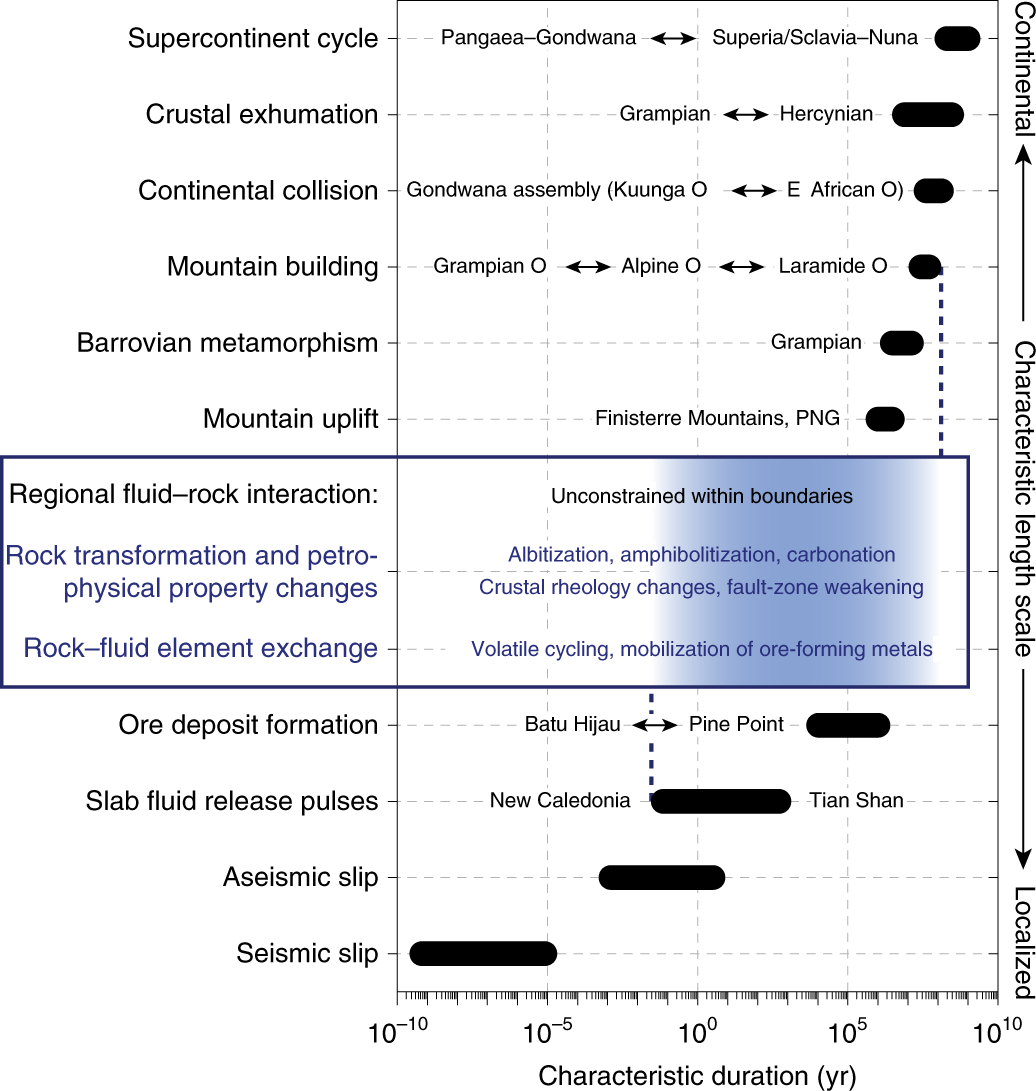
\includegraphics[width=0.5\linewidth]{figures/fig1.png}
	\caption{\textbf{Characteristic durations and scales of geological processes}.The durations of fluid–rock interactions remain unconstrained between orogenic processes and fluid release from subducting slabs. Data are compiled from: supercontinent cycle43, crustal exhumation44,45, continental collision12, mountain building13,14, Barrovian metamorphism46, mountain uplift47, ore deposit formation48,49, slab fluid release15,16 and seismic and aseismic slip50. E, East; O, orogeny; PNG, Papua New Guinea.}
	\label{fig:fig1}
\end{figure}

To quantify fluid–rock interaction durations, the feasible fluid advection velocities through the crust must be known. However, the small dimension of intra-crustal fluid pathways hampers a direct geophysical monitoring, and forward simulations based on extrapolating the measured rock permeability are subject to large uncertainties that arise from transient variations, such as those documented for shallow seismic events and geothermal system stimulations\cite{John2012,Hanson1992,ingebritsen2010permeability}. Furthermore, such transient variations probably also occur in the deeper crust, as inferred from preserved pore networks in exhumed metamorphic rocks, numerical simulations and time-integrated fluid-flux calculations\cite{ingebritsen2010permeability,manning1999permeability,Plumper2017,Bickle1990,Skelton2011}.

Therefore, to quantify the duration of regional-scale fluid–rock interactions, here we first investigated the exceptional exposure of abundant and clearly defined, sharp reaction fronts that result from the fluid-driven alteration of serpentinite. These field relationships provide critical insights into the conditions and geometry of fluid migration, and the relatively simple composition of the ultramafic precursor offers a reduced complexity compared to that of other large multicomponent natural systems. Then, using the obtained parameters, we constrained the duration of fluid–rock interaction by fitting an innovative numerical model that couples reactive transport, mass conservation and local equilibrium thermodynamics with the mineral chemistry and abundance, and the composition of the hydrothermally altered rock.

\section*{Serpentinite alteration by reactive fluid flow}

Our natural laboratory comprises a tectonically dismembered ophiolite situated within greenschist-to-lower amphibolite facies metamorphosed metasediments of the Caledonian Köli Nappe of northern Norway (Methods)3,28. About 20 individual ophiolite fragments are pervasively altered to a talc–magnesite–chlorite assemblage (soapstone) on the scale of several hundred cubic metres due to their reaction with carbon-bearing aqueous fluid28. Reaction fronts are sharp on both the outcrop and the thin section scales, and they are defined by the formation of the soapstone assemblage from a completely serpentinized precursor (Figs. 2a and 3a,b, Extended Data Fig. 1 and Supplementary Fig. 1). The presence of pervasively carbonated contact zones between the ophiolite and the underlying sedimentary schist indicates a local origin of the alteration fluid (Fig. 2b)28, in which a carbon-bearing aqueous pore fluid is released due to the compaction of the local sediments and/or the thermally facilitated dissolution of carbonate during tectonic underthrusting below the relatively hotter oceanic lithosphere (Fig. 2b)29. Additional soapstone is present in reaction selvages along intra-ophiolite fractures that are ten to several hundred metres long and connected to the basal thrust, indicating the fractures functioned as fluid conduits (Fig. 2b). Importantly, one of these reaction selvages perfectly exposes the field relationships, which allowed us to extract the necessary parameters at the required precision to constrain the fluid–rock interaction timescale via modeling (Extended Data Fig. 1).

\begin{figure}[ht]
	\centering
	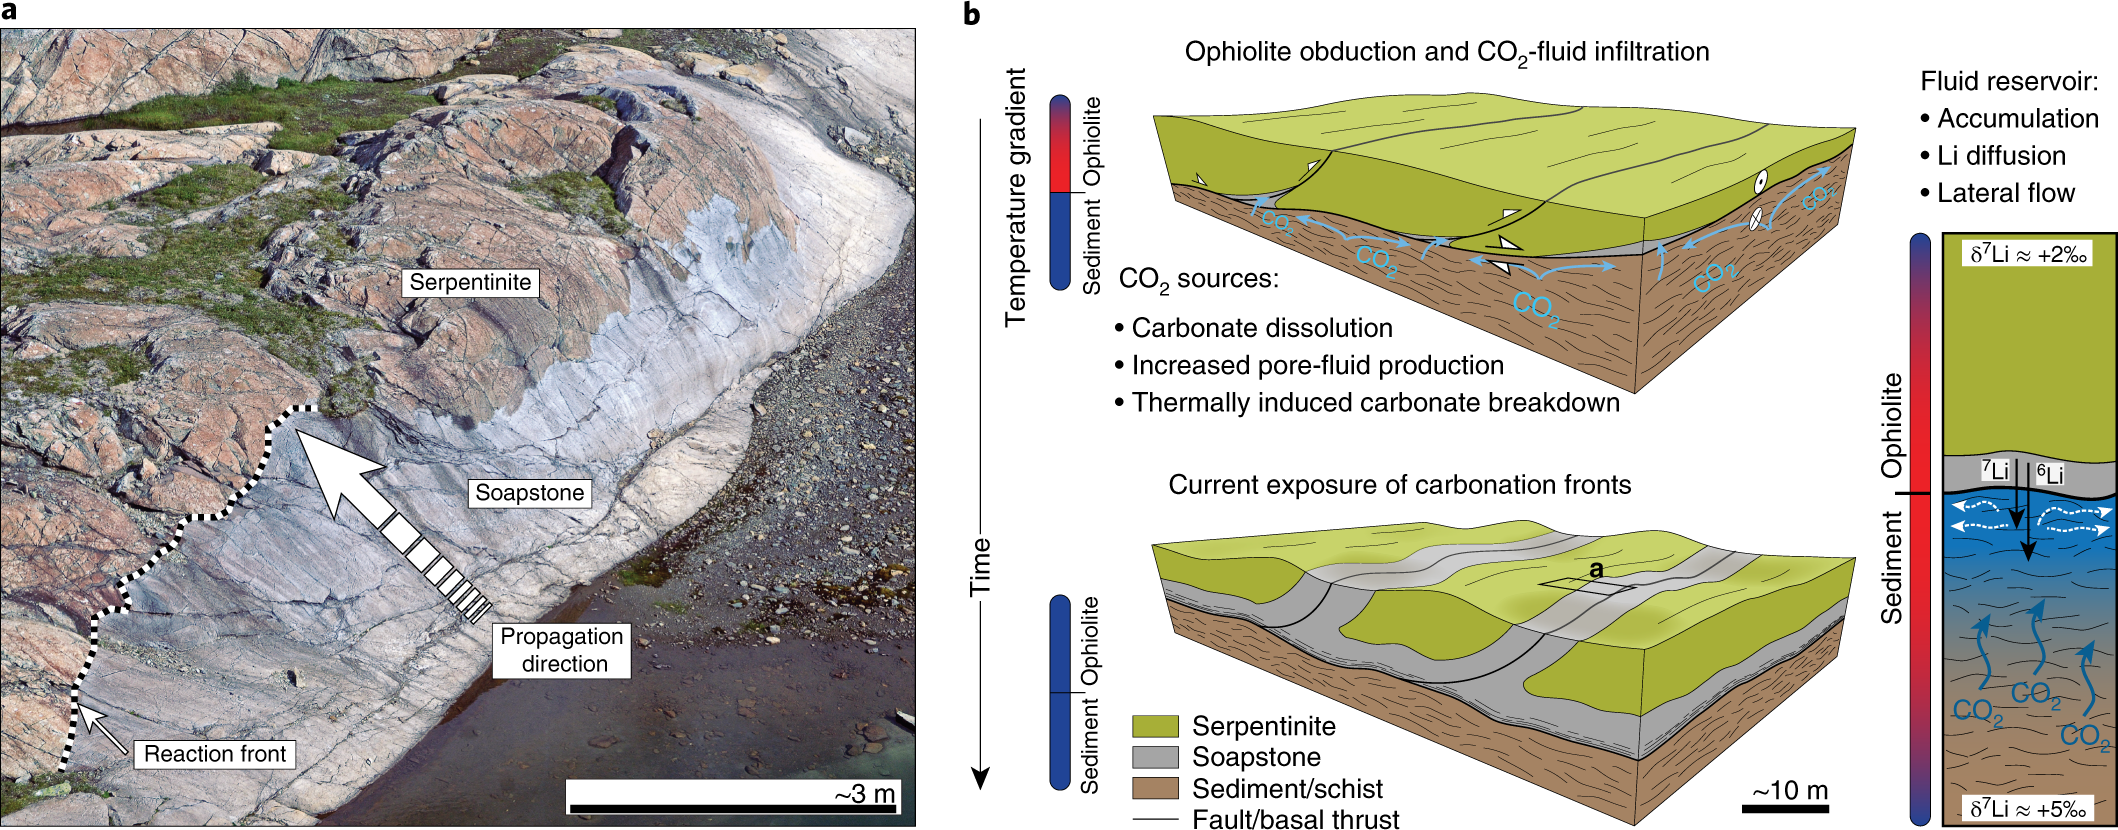
\includegraphics[width=0.5\linewidth]{figures/fig2.png}
	\caption{\textbf{Ophiolite obduction and alteration.}a, Representative outcrop image of a ~3 m wide soapstone alteration selvage around a fracture in serpentinite. b, Schematic depicting ophiolite emplacement onto metasediments, alteration fluid accumulation below the basal ophiolite thrust and soapstone formation along the thrust and fluid conduits. Lithium isotope exchange during incipient alteration across the tectonic contact controls the lithium budget of the alteration fluid reservoir. The temperature gradients illustrate the thermal evolution of the system during and after ophiolite obduction and alteration.}
	\label{fig:my_label}
\end{figure}

\begin{figure}[ht]
	\centering
	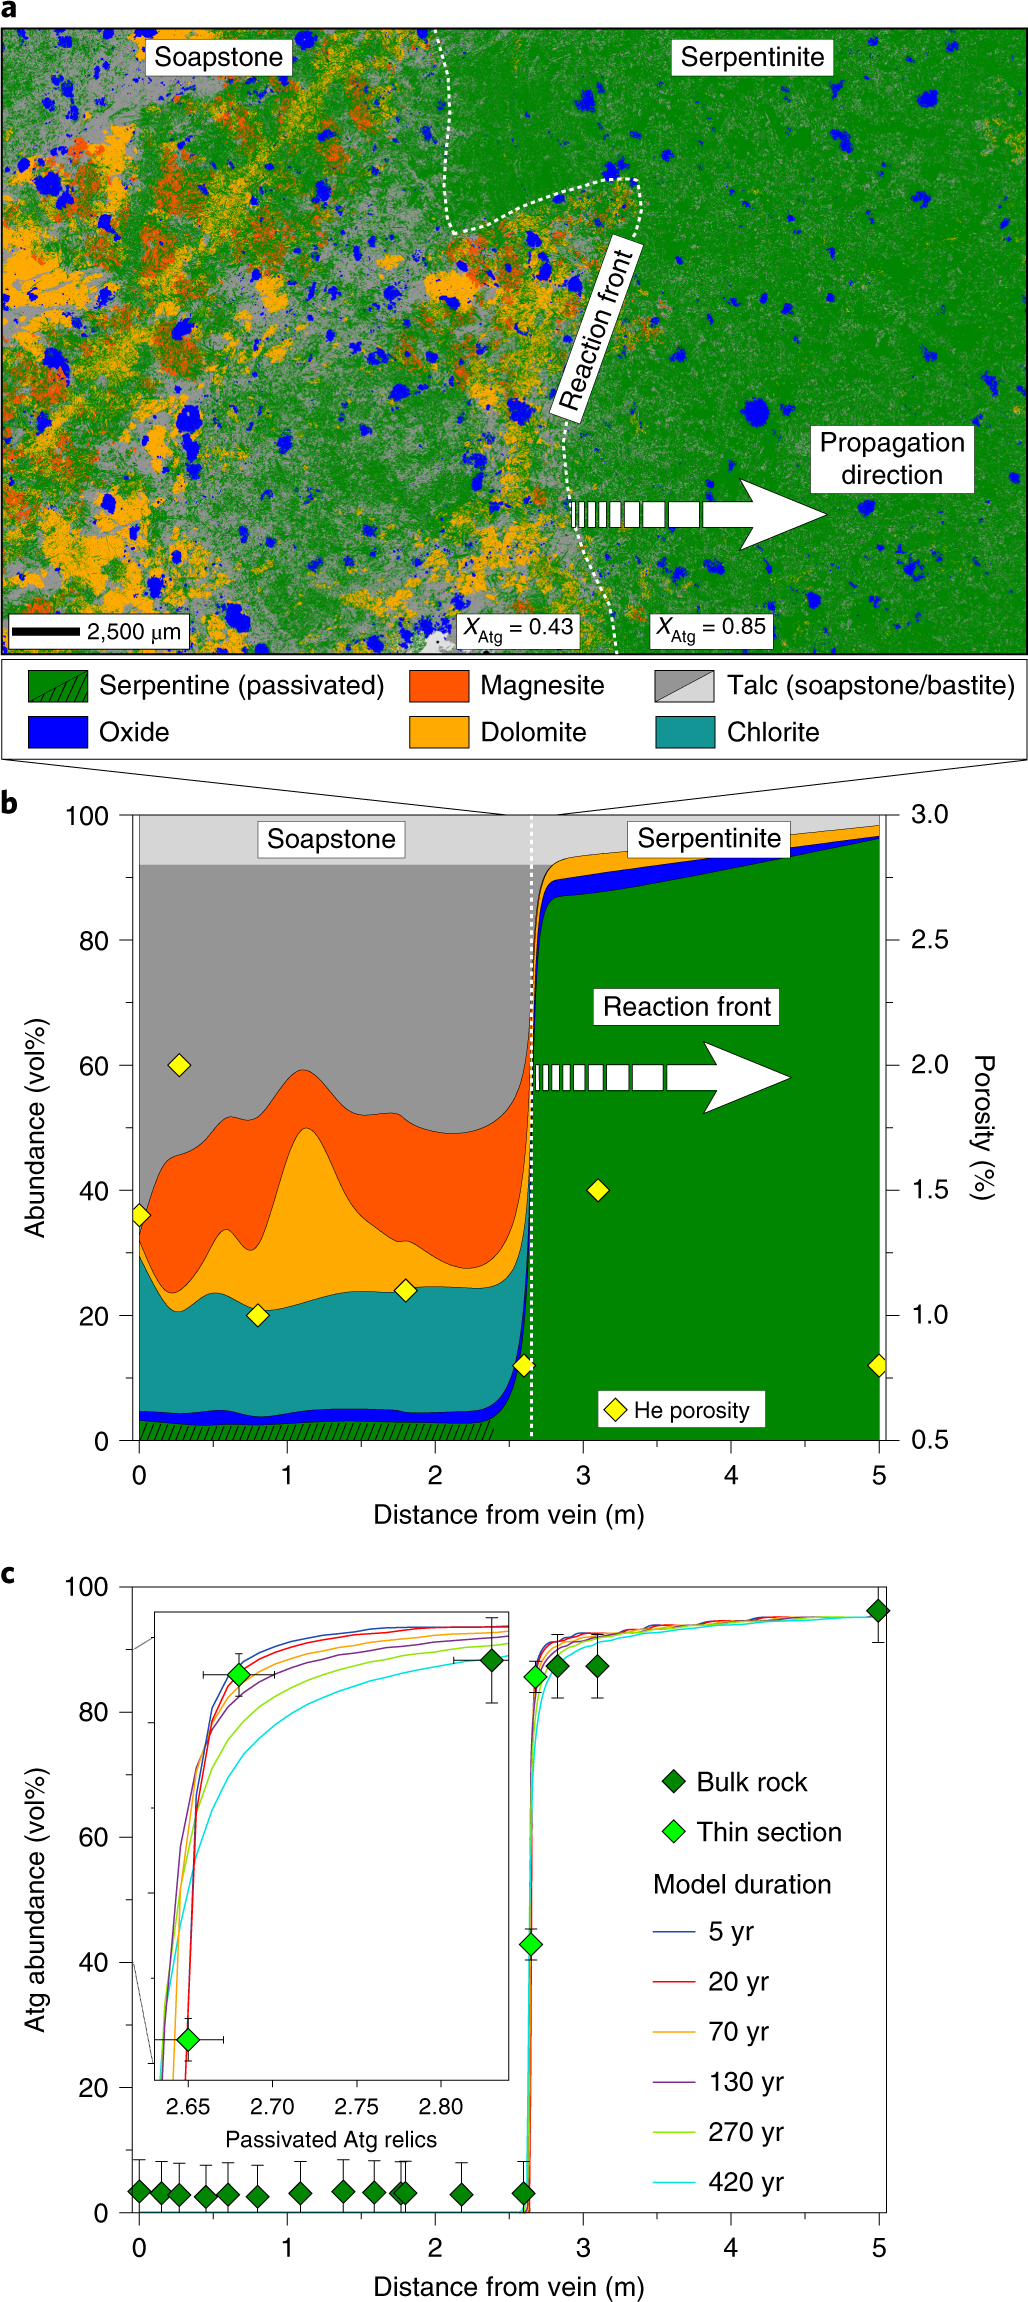
\includegraphics[width=0.5\linewidth]{figures/fig3.png}
	\caption{\textbf{Mineral replacement during serpentinite alteration.}a, Mineral distribution map across the reaction interface. b, Bulk rock mineral abundance across the reaction interface. Talc in serpentinite is a relic from earlier pyroxene. Serpentine in soapstone occurs as inclusions in magnesite (Supplementary Fig. 1c). c, The reactive transport model fitted to measured antigorite volume fractions for different alteration durations. Vertical error bars denote a 10\% uncertainty of the bulk rock data and a 5\% uncertainty of the thin section data. The uncertainty of the measured sample locations is the drill core diameter. The distance uncertainty of the thin section data is the half-width from each end. Atg, antigorite.}
	\label{fig:fig3}
\end{figure}

Our observations and model input parameters are based on the analyses of 17 core samples from a 5 m long transect across a 2.6 m wide soapstone fracture selvage in serpentinite (Extended Data Fig. 1). The texturally and compositionally homogeneous soapstone contains on average 29 ± 5 vol\% carbonate dominated by magnesite, 17 ± vol\% chlorite and 48 ± 5 vol\% talc (Supplementary Methods 2). The modal contents of magnetite and relic serpentine inclusions in carbonate are below 3 vol\% (Fig. 3b, Supplementary Figs. 1 and 2 and Supplementary Tables 1 and 2). A lithostatic pressure of ~300 MPa is inferred from the alteration temperature of ~300 °C (ref. 28) and a thermobaric gradient of ~1 °C MPa−1.

\section*{Reactive transport local equilibrium model}

In our numerical model, serpentinite is replaced by soapstone along the one-dimensional (1D) fluid infiltration path perpendicular to the central fracture in response to the advective–diffusive transport of carbon, silica and lithium through interconnected pore space (Fig. 3c, Methods and Extended Data Fig. 1). The carbon concentration of the input fluid is low (CO2 ~1 wt\%), consistent with the composition of natural fluids, thermodynamic predictions and experimental observations28,30,31, and aqueous silica is derived from serpentine dissolution along the flow path. Changes of fluid and solid compositions are controlled by mineral replacement in accordance with local equilibrium thermodynamics and mass conservation. Thus, mineral proportions and chemistry vary in response to the dynamically changing system composition, and the model reproduces the observed mineral proportions and compositions (Methods). Using the known diffusion coefficient, fluid and rock densities, and length scales, we minimized the mismatch between the observed and modelled data, and thus reproduced the observed front sharpness by varying the advective fluid flux relative to carbon diffusion in the aqueous fluid. Generally, a faster fluid advection increased the sharpness and propagation rate of the reaction front. This unique approach constrains the alteration duration to $20\pm \frac{9}{5}$
years, equivalent to a surprisingly fast average front propagation rate of ~0.13 m yr−1 (Fig. 3c; see Methods for the discussion of the model uncertainty). The obtained front propagation rate is orders of magnitude faster than that inferred from retrograde metamorphic reactions at high temperature but fluid-starved conditions19 and is at least as fast as the fastest current tectonic plate motion.

\section*{Constraints from Li isotope systematics}
This calculated duration of the reaction front propagation is consistent with the measured variation of bulk rock lithium concentrations and isotope ratios (δ7Li), which are known to accompany short fluid–rock interaction processes15,16. Lithium concentrations in the soapstone gradually decrease from the reaction interface towards the vein, whereas lithium isotope ratios are high near the vein (δ7Li = 4.9‰), slightly lower in the precursor serpentinite (δ7Li ≤ 2.2‰), and show a significant deviation to negative values (δ7Li = −4.5‰) in the centre of the reaction selvage (Fig. 4a and Supplementary Table 3). Lithium solid-state diffusion is slow at mid-crustal temperatures. Hence, the outcrop-scale variation in lithium isotope ratios can only result from the faster diffusivity of 6Li relative to 7Li during fluid-mediated transport after lithium is released from antigorite, but before lithium is taken up by secondary chlorite and talc. However, the mass transport efficiency during reactive fluid flow is controlled by the fluid–solid mass transfer. Elements that more strongly partition into the solid are chemically retarded relative to those that partition less strongly into the solid. Available partition coefficients indicate that lithium concentrations are generally lower in the solid than in the respective equilibrium fluid, whereas measured carbon concentrations in the soapstone are approximately ten times higher than those in the equilibrium fluid (Extended Data Fig. 2a and Supplementary Methods 3.1). Hence, carbon transport and propagation of the reaction front are retarded relative to the transport of lithium, and lithium released by the reaction at the front will be transported downstream instead of being incorporated in talc and chlorite. Consequently, the observed systematic trend in the δ7Li variation over time can only reflect fluid compositional changes that are controlled by reactions outside the sample transect that occur at large scales (Fig. 4b,c). In contrast to the relatively small-scale fracture reaction selvages within the ophiolite, the fluid–rock interaction occurs on a much larger scale along the tectonic contact with the underlying sedimentary schist, where we observe consistently pervasive thrust-parallel soapstone alteration (Fig. 2b, Methods and Extended Data Fig. 5). Predominantly horizontal fluid reservoir drainage into the tectonic fluid conduits within the ophiolite has only a minor influence on the composition of the alteration fluid (Fig. 4c). Thus, we attribute the variation of δ7Li along the investigated transect to a large-scale diffusive lithium exchange between the antigorite dehydration fluid and the sediment-hosted fluid (Fig. 4a).

\begin{figure}[ht]
	\centering
	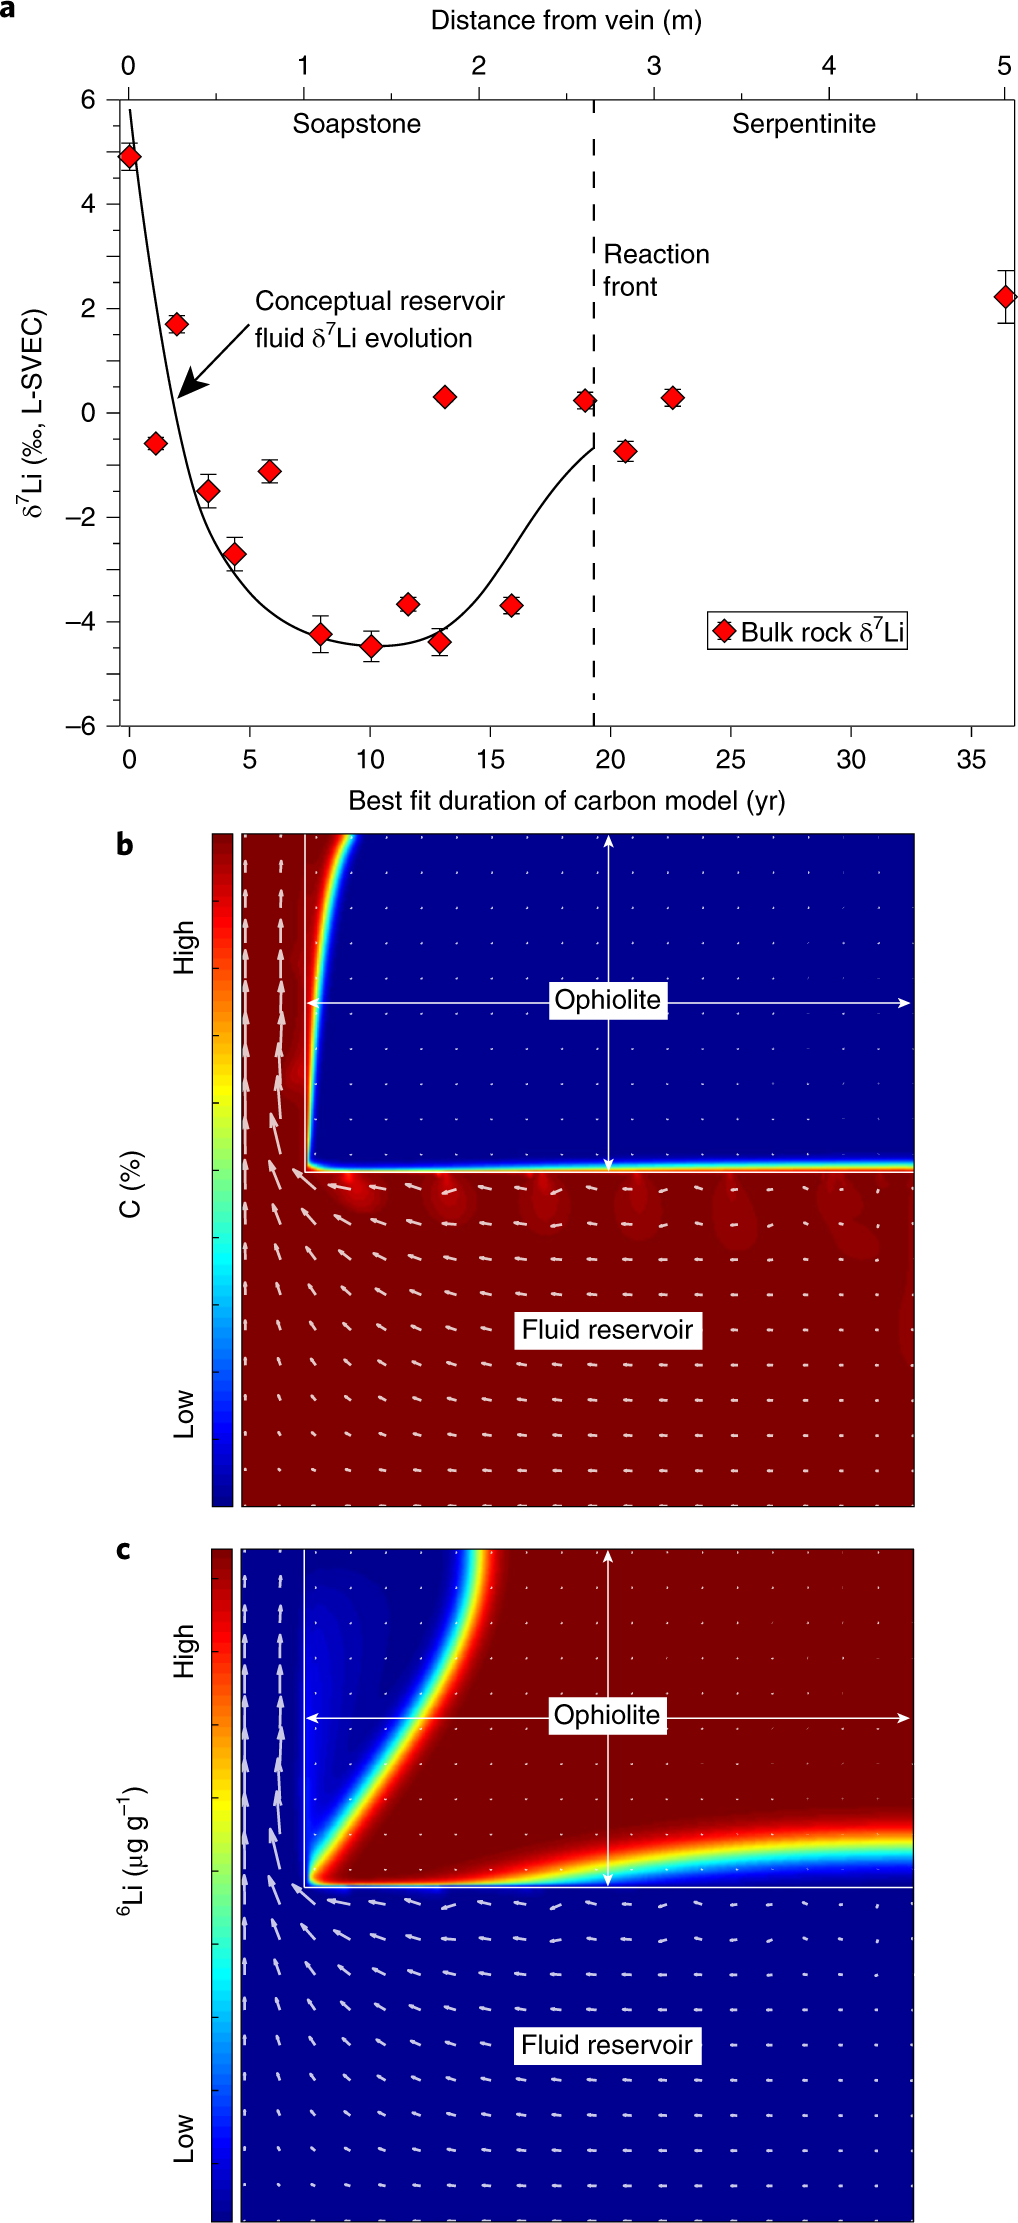
\includegraphics[width=0.5\linewidth]{figures/fig4.png}
	\caption{\textbf{Outcrop lithium isotope distribution and fluid reservoir compositional evolution.}a, Bulk rock lithium isotope distribution in outcrop and conceptual reservoir fluid δ7Li evolution during diffusive isotope exchange between the ophiolite- and sediment-hosted alteration fluid (see also panel c, Fig. 2b and Extended Data Fig. 5). The bottom abscissa shows the timescale obtained from the reactive transport model. Error bars indicate the 2σ analytical uncertainty. b, Fluid carbon concentrations and flow vectors in 2D. Beneath the basal thrust, flow is predominantly horizontal and drains the top section of the fluid reservoir into the ophiolite-hosted vertical fracture. Fluid density gradients result in deviation from a purely horizontal flow. c, Fluid 6Li concentrations in 2D, showing that mineral replacement lags behind the fluid 6Li front.}
	\label{fig:fig4}
\end{figure}

\section*{Consequences of fast reaction front propagation}
Another intriguing aspect of the modelling approach is that it allows us to evaluate the implicitly changing permeability based on a simple Darcy relationship and assuming a buoyancy-driven hydraulic gradient (∇P = g × (ρfluid – ρsolid)) of about −19 MPa km−1 (ref. 24). The model input flux that results in the best fit of the modelled-to-measured antigorite abundance (equivalent to the fluid–rock interaction duration of ~20 years) is 20.4 m yr−1. This implies a permeability, κ, of ~10−14.5 m2 during the reaction front propagation, which is high compared to the measured permeability of the least-carbonated serpentinite of ~10−17 m2 (Supplementary Table 2) and that of antigorite from another location (κ ≈ 10−20 m2) (ref. 32). However, similarly high values have been hypothesized to occur transiently during fluid-driven metamorphic reactions despite the lack of robust timescale constraints23. Fitting the modelled-to-measured antigorite abundance by using the measured permeability (κ ≈ 10−17 m2) requires an unrealistically strong hydraulic gradient, ~2.5 orders of magnitude higher than that derived from the fluid–solid buoyancy contrast. Hence, we interpret the calculated permeability as a transient, reaction-induced corollary of front propagation.

The presence of abundant and large-scale soapstone alteration within an area of ~70 km2 (ref. 28) indicates a pervasive fluid–rock interaction at the regional scale, facilitated by the concomitant alteration at multiple structurally controlled reaction zones. Soapstone–serpentinite fronts are consistently sharp throughout the entire field area, and front propagation distances from identifiable fluid conduits typically vary between a few centimetres and several tens of metres, but the fronts lack evidence for repeated fluid infiltration, such as overprinting of pre-existing fronts and cross-cutting relationships. Hence, we infer that the calculated front propagation velocity (0.13 m yr−1) is also applicable at the field scale, which implies a regional-scale alteration duration on the order of 10–100 years. The parameters of our numerical simulation are consistent with the background permeability, fluid composition and pressure and temperature conditions of the deeper crust irrespective of local lithology. Moreover, in our model hydrous serpentinite is altered by an aqueous fluid that contains ≤1 wt\% CO2 and the rock alteration driving force is probably higher for the alteration of anhydrous high grade metamorphic and igneous rocks with aqueous and ore forming hydrothermal fluid8,11,33,34. Hence, the characteristic timescale of fluid–rock interaction in such systems may be even shorter and may further decrease at higher temperatures in the lower crust.

Our data indicate that fluid-mediated rock alteration fronts propagate at least at the same rate as large-scale tectonic processes, including mid-ocean ridge spreading, plate motion and subduction35,36,37. Consequently, fluid-mediated changes in the physical properties of rock also proceed, from a geodynamic perspective, instantaneously. This not only has important implications for the rates of rheology, gravity and magnetic character changes of the newly formed oceanic lithosphere exposed to hydrothermal seawater circulation along mid-ocean ridges3,5,38, but also justifies the assumption of instantaneous rock equilibration in large-scale geodynamic models that link, for example, far-field crustal deformation to differences in rheologic properties2,39,40. Moreover, fast fluid–solid reactions may explain the progressive propagation of tectonic relaxation fronts and the transient nature of episodic tremor and slip that have been related to localized near-lithostatic fluid pressure41,42. Our data directly show that carbon uptake in ultramafic rock takes place on timescales of tens to hundreds of years. If ophiolites are repeatedly infiltrated by carbon-bearing fluid over a sufficiently long timescale, they may represent effective sinks in the long-term carbon cycle. Finally, if the timescales of hydrothermal ore deposit formation are equally short, fluid–rock interactions actively recharge the crustal endowment in mineral commodities on timescales relevant for the resources demand of future generations.

\section*{Methods}

\subsection{Geological context and field relationships}
The Linnajavri field area is centred around 67° 36′ N and 16° 24′ E and contains ~20 individual ultramafic bodies distributed over an area of ~70 km2 (ref. 51). The area of individual ultramafic bodies, as exposed at the surface, ranges between several 100 m2 to a few km2. In the field, ultramafic bodies cluster in both a northern and a southern zone, the former of which is part of the Čohkul Nappe and contains the investigated outcrop, whereas the southern zone is part of the Ridoalggičohkka Nappe. In the Ridoalggičohkka Nappe, ultramafic rocks are underlain by carbonate–mica schist and subordinate calcite–dolomite marble, thin layers of quartzite, garnet-bearing mica schist and semi-concordant trondhjemite sills. The northern Čohkul Nappe is composed of garnet–mica schist and metagreywacke. Both nappes are gently folded and most of the ultramafic bodies are present in the central parts of large synclinal structures51. Both local nappes are part of the regional Köli Nappe, which has been described as a sequence of Cambrian to Silurian oceanic metasediments that comprise calcareous psammite and pelite. The Köli Nappe is part of the Upper Allochthon of the Caledonian tectonostratigraphy52,53. In a few other places, the Köli Nappe has been further subdivided into several subunits and in these other sites ophiolite fragments are typically found in the lowermost subunits above the contact with the underlying Seve Nappe54. The metamorphic grade of the Köli Nappe is mostly greenschist facies and an upward increase to lower amphibolite facies has been documented from the Nordhallen area of west-central Sweden54,55.

The least-altered rock type in all the investigated ultramafic bodies is serpentinite and primary pyroxene and olivine have not been found3,28,51. The northern zone contains soapstone and serpentinite and the southern zone contains additional mafic rocks, which include pillow basalts, and listvenite along the basal thrust of the ultramafic bodies, that is, the quartz–magnesite alteration assemblage. The alteration of serpentinite to soapstone and listvenite is consistent with the infiltration of a carbon-bearing reactive fluid and does not require additional silica and other components3,9,28,56,57. Based on a conservative depth extrapolation, the total volume of soapstone at Linnajavri has been estimated as ~100 Mt but may be 2–3 times larger51. The alteration features and composition of serpentinite and soapstone are consistent throughout the field area. Serpentinite alteration is most strongly developed along the basal thrust of the ultramafic bodies and can be followed along fractures as reaction selvages into the interior parts of the ultramafic bodies. The reaction fronts shown in Fig. 2a and Extended Data Fig. 1 are representative of the front sharpness in the entire field area. In the field, soapstone can appear grey and rust brown, the latter of which is attributed to a more intense weathering and less mechanical erosion during the recent glaciation of the area. However, surface weathering is restricted to the outermost ~5 mm and the soapstone composition is invariant below the weathered surface. Despite the small degree of surface weathering, the location shown in Extended Data Fig. 1 was chosen for this study as it most clearly shows the relationship between the fluid conduit, alteration selvage and precursor serpentinite, and allowed for precise distance measurements.

\subsection*{Local equilibrium thermodynamic model}
The multicomponent ultramafic system is approximated in the SiO2–Al2O3–MgO–FeO–CaO–H2O–CO2 compositional space. Phase equilibria were calculated for 300 °C and 300 MPa, consistent with the previous temperature estimate and a geothermobaric gradient of 1 °C MPa−1 (ref. 28). Furthermore, all the calculations were conducted using the system composition specified by element concentrations. To define a subspace of the entire compositional spectrum for the thermodynamic calculations, we precomputed all the possible compositional variations that may result from the fluid–rock interaction and subsequently focused on the relevant reactions that are informed by field observations and sample petrography. The critical reaction for the formation of soapstone from serpentinite is the dissolution of antigorite during the addition of CO2 to form magnesite and talc:

\begin{equation}
	dsjflds
	\label{eq:eq1}
\end{equation}

Furthermore, the absence of quartz provides an upper limit for the alteration-fluid carbon concentration, above which serpentine alteration would form the assemblage magnesite + quartz (listvenite)28. Sample petrography also defines the composition of the starting material as a mixture of antigorite and dolomite without additional fluid (Lin\_31; Supplementary Tables 1 and 2)28. Based on this composition, the critical elements that vary by dissolution and solute transport are carbon and silica. Hence, the compositional space is reduced to 2D. Charge balance constrains the amount of oxygen in the bulk composition, assuming all the Fe is ferrous, consistent with the absence of haematite and goethite from the samples.

For the calculations, we used solid-solution models for olivine (O(HP)), spinel (Sp(HP)), antigorite (Atg(PN)), brucite (B), magnesite (M(HP)), talc (T), chlorite (Chl(HP)), dolomite (Do(HP)), clinopyroxene (Omph(GHP)) and amphibole (Amph(DPW))58,59,60,61,62 together with the thermodynamic dataset of Holland and Powell58. For the fluid phase we used the H2O–CO2 mixing model by Aranovich and Newton63 with the H2O and CO2 endmembers derived from the CORK EOS of Holland and Powell64. This model was extended to include the aqueous silica endmember58, which closely reproduced the quartz solubility experiments65. The mixing with aqueous silica was only done for the dilute limit in which we took an ideal mixing approximation. Recent experimental evidence indicates that this modelling approach very closely reproduces phase equilibria in ultramafic systems in the presence of C–O–H fluids31. All the calculations were done in MATLAB following the methodology described in Vrijmoed and Podladchikov66 and Plümper et al.67.

We calculated the change in system composition and mineral abundance by independently varying the concentration of carbon between 0 and 1 mol\% (Extended Data Fig. 2). Both the bulk system composition and the mineral abundance gradually changed with increasing carbon content, so that modes of talc and magnesite increased with decreasing antigorite content and chlorite stabilizes at a high carbon content just before antigorite reacted out. Our model accurately reproduces measured mineral compositions (Extended Data Fig. 3)28. The concentration of the system components in individual phases with increasing bulk system carbon content is shown in Extended Data Fig. 4. The thermodynamic calculations thus yield bulk rock and fluid densities, total volatile (CO2 + H2O) weight fractions in the solid and bulk solid carbon concentration for the T, P, Cfluid space of interest. These are the local thermodynamic closing relations for the reactive transport calculation, as discussed below.

\subsection*{Reactive transport model}

The advection–diffusion–reaction model is based on local thermodynamic equilibrium and mass conservation at the propagating replacement front. Replacement of serpentinite by soapstone proceeds as a coupled carbonation and partial dehydration reaction. The conservation of both fluid and solid mass is expressed as:

\begin{equation}
	\frac{\partial }{{\partial t}}\left( {\rho _{\rm{f}}\phi + \rho _{\rm{s}}\left( {1 - \phi } \right)} \right) + \nabla \left( {\rho _{\rm{f}}\phi {\bf{V}}_{\rm{f}} + \rho _{\rm{s}}\left( {1 - \phi } \right){\bf{V}}_{\rm{s}}} \right) = 0
	\label{eq:eq2}
\end{equation}

\noindent where ρs is the solid density, ρf the fluid density, ϕ the fluid-filled porosity, Vf the fluid velocity and Vs the solid velocity. The conservation of immobile solid mass is implemented by using:

\begin{equation}
	\frac{\partial }{{\partial t}}\left( {\rho _{\rm{s}}(1 - C_{\rm{s}}^{\rm{m}})\left( {1 - \phi } \right)} \right) + \nabla \left( {\rho _{\rm{s}}(1 - C_{\rm{s}}^{\rm{m}})\left( {1 - \phi } \right){\bf{V}}_{\rm{s}}} \right) = 0
	\label{eq:eq2}
\end{equation}
%
%\bibliography{refs.bib}
%\bibliographystyle{gmd}

\end{document}
